%% TODO: Add a small paragraph to tell what this chapter is about
This chapter delves into the implementation of each module inside Test Genie system. Overall, this system consist of three main modules: 
\begin{itemize}
    \item[-] \textbf{Project Manager}: This module manages all the projects that are cloned to server. It mostly responsible for file-based activities and running CLI for each project.
    \item[-] \textbf{Business Logic Analyzer}: This module will take various source file from Project Manager and break the source code into smaller pieces (blocks). Then, it will analyze each block and determine what each block does and how it should be tested if possible. A test plan will also be generated for each block and save it to the database.
    \item[-] \textbf{Test Generator}: This module will take the test plan from Business Logic Analyzer and generate a test case for each block. The generated test cases will be saved as files directly in the project source code on server and can be used to run the tests later (validation).
\end{itemize}
Additionally, this system also have \textbf{DBMS} module to control the database but this module will not be explained thoroughly in this chapter.

%% TODO: Make sure to use \textbf or \textit for highlighting keywords, and \cite{} to cite the corresponding quotations

\section{Project Manager module}

The \textbf{ProjectManager} module serves as the core backend functionality for handling projects within the Test Genie system. It provides a robust framework for managing software projects by integrating Git-based repositories, file management, and testing workflows. The module is built around the \textit{Project} class, which encapsulates essential functionalities such as cloning repositories, recognizing project frameworks, and managing project files. Additionally, it features an abstract interface for test creation, validation, and execution, allowing for framework-specific extensions of functionality. For instance, the \textit{Flutter} subclass extends the \textit{Project} class to handle Flutter-specific tasks, including dependency management, `pubspec.yaml` parsing, and test execution. By modularizing these functionalities, the \textbf{ProjectManager} module streamlines project handling and enhances the system's scalability for various software development frameworks.

\subsection{Module prequisites}
This module require the SDK of supported frameworks to be installed standablone in folder \textit{./SDKs} inside the module folder. This design not only allows the module to be easily extended and modifiled to support other frameworks, but also avoid more SDK installation on the server OS. Since the \textit{Project} class (Listing A.1) just mainly control git management and file management, the subclass can freely control how the SDKs are used. \\

Subclass of Project are required to implement the following methods:
    \begin{itemize}
        \item[-] \textbf{create\_test}: This method will create the test file in the location that is required by the framework.
        \item[-] \textbf{get\_test\_content}: This method will return the content of the test file that is created by the \textbf{create\_test} method. The content of the test file is generated by the Business Logic Analyzer module.
        \item[-] \textbf{run\_test}: This method will run the test file that is created by the \textbf{create\_test} method. The test result will be returned to the caller.
        \item[-] \textbf{validate}: This method will run all the test files in the test directory and return the result. This method is used to validate the test files that are created by the \textbf{create\_test} method.
        \item[-] \textbf{getListSourceFiles}: This is an important method, which will partly decide how the source code is split into blocks. The starting point file (main file) should be placed on the first position of the list. The list will be used to split the source code into blocks. The list should contain all the source files in the project (relative to the project directory).
    \end{itemize}


\subsection{Flutter class}

The \textbf{Flutter} class extends the \textbf{Project} class to provide framework-specific support for managing Flutter projects. This class is responsible for handling operations unique to Flutter, such as managing dependencies, running tests, and validating projects. It ensures that the Flutter SDK is installed and properly configured in the \textit{./SDKs/flutter} directory before performing any operations.

Key methods of the \textbf{Flutter} class include:
\begin{itemize}
    \item[-] \textbf{\_runFlutterCLI}: This method executes commands using the Flutter CLI within the context of the project directory. It supports arguments for various Flutter commands and handles errors if the command fails.
    \item[-] \textbf{\_checkSDK}: Ensures that the Flutter SDK is installed and operational by running the \texttt{flutter --version} command. If the SDK is not present or misconfigured, the method raises an exception.
    \item[-] \textbf{\_flutterPubGet}: Automatically installs dependencies listed in the \textit{pubspec.yaml} file by running \texttt{flutter pub get}.
    \item[-] \textbf{\_addTestDependency}: Adds the Flutter \textit{test} package as a dependency using \texttt{flutter pub add test}.
    \item[-] \textbf{create\_test}: Creates a test file in the designated \textit{test} directory of the project. If the file already exists and overwriting is not allowed, an exception is raised.
    \item[-] \textbf{get\_test\_content}: Retrieves the content of a test file from the \textit{test} directory.
    \item[-] \textbf{run\_test}: Executes a specified Dart test file using the Flutter CLI and returns the results.
    \item[-] \textbf{validate}: Iterates through all Dart test files in the \textit{test} directory and validates them by running each test.
    \item[-] \textbf{getListSourceFiles}: Collects and returns a list of all source files in the \textit{lib} directory, ensuring that the \textit{main.dart} file is prioritized as the entry point.
\end{itemize}

This design enables seamless integration of Flutter-specific features into the \textbf{Test Genie} system while adhering to the modular structure defined by the \textbf{Project} class. By implementing these methods, the \textbf{Flutter} class ensures compatibility with the broader system and provides developers with a streamlined process for managing and testing Flutter projects.

\section{Business Logic Analyzer module}

The \textbf{Business Logic Analyzer} module is designed to parse and analyze the source code of a project. It constructs a \textbf{Dependency Diagram} that represents the logical structure and relationships within the project. By leveraging framework-specific analysis strategies, such as the \textit{FlutterAnalyzeStrategy}, this module identifies functional blocks and their interconnections. Each block is further enriched with predictions generated by the \textbf{AI Agent}, which analyzes the code to provide insights into its behavior and logic. This modular design allows the Business Logic Analyzer to be easily extended to support additional frameworks, making it versatile and scalable for various software projects. The output of this module serves as the foundation for the subsequent test generation process.

\subsection{DependencyDiagram class}

The \textbf{DependencyDiagram} class serves as a connector within the Test Genie system, bridging the gap between the framework-specific analysis strategies, such as \textit{FlutterAnalyzeStrategy}, and the AI-powered prediction functionality provided by the \textbf{AI\_Agent}. This class is responsible for constructing a logical representation of the project in the form of a dependency diagram, which comprises blocks (representing functional units) and connections (representing the relationships between those units). The \textbf{\_generateDiagram} method encapsulates this functionality by invoking the appropriate analysis strategy for the project's framework (Listing A.3), allowing the class to dynamically adapt to diverse frameworks supported by the system. This modular design ensures that the class is both extensible and maintainable as new frameworks are introduced.

In addition to structural analysis, the \textbf{DependencyDiagram} class leverages the \textbf{AI\_Agent} to enrich the diagram with meaningful predictions. Through the \textbf{\_getPre-dictions} method (Listing A.3), each block in the diagram is analyzed to generate insights into its behavior and logic, which are subsequently embedded into the block. This integration of AI-based predictions and static code analysis makes the \textbf{DependencyDiagram} a powerful tool for understanding the project's overall architecture and behavior. By combining these two mechanisms, this class plays a pivotal role in preparing the business logic analyzation for further steps in the Test Genie system: test generation and validation.

\subsubsection{Diagram objects}


The DependencyDiagram class relies on objects from the Diagram folder to represent the blocks and connections within the dependency structure. These objects are defined as follows:

\begin{itemize}
    \item[-] \textbf{Block class}: Represents the functional units of the source code, such as files, classes, functions, or variables (Listing A.4). Each block contains the following attributes:
    \begin{itemize}
        \item[-] \textit{name}: The name of the block.
        \item[-] \textit{content}: The source code or content of the block.
        \item[-] \textit{type}: The type of the block, determined by the BlockType class.
        \item[-] \textit{prediction}: (Optional) AI-generated predictions for the block's logic or behavior.
    \end{itemize}
    Additionally, the Block class provides methods such as:
    \begin{itemize}
        \item[-] \textbf{getContentNoComment}: Removes comments from the block's content for clean analysis.
        \item[-] \textbf{setPrediction} and \textbf{getPrediction}: Manage predictions for the block.
    \end{itemize}

    \item[-] \textbf{BlockType class}: Enumerates the possible types of blocks (Listing A.5), such as \textit{File}, \textit{Class}, \textit{Function}, and more. It also provides methods to:
    \begin{itemize}
        \item[-] Generate database queries for storing and managing block types.
        \item[-] Define the schema for the BlockType database table.
    \end{itemize}

    \item[-] \textbf{Connection class}: Represents relationships between blocks (Listing A.6), with attributes:
    \begin{itemize}
        \item[-] \textit{head}: The source block of the connection.
        \item[-] \textit{tail}: The destination block of the connection.
        \item[-] \textit{type}: The type of relationship, determined by the ConnectionType class.
    \end{itemize}
    It also facilitates database storage and retrieval through schema definitions.

    \item[-] \textbf{ConnectionType class}: Enumerates the types of relationships between blocks (Listing A.7), such as \textit{Extend}, \textit{Implement}, \textit{Call}, and \textit{Import}. It provides similar database-related methods as the BlockType class.
\end{itemize}

\subsubsection{FlutterAnalyzeStrategy Algorithm}

The \textbf{FlutterAnalyzeStrategy} function (Listing A.8) is a core component of the \textbf{DependencyDiagram} generation process within the \textbf{Business Logic Analyzer} module. This function is specifically designed to analyze Flutter projects by reading their source code, breaking it into logical units (\textit{blocks}), and appending these blocks to the diagram. It employs three custom backtracking algorithms (\textit{ImportAnalyzer}, \textit{ContainAnalyzer}, and \textit{CallAnalyzer}) to achieve a comprehensive structural and relational analysis of the project. Here's a detailed breakdown of the algorithm:

\begin{itemize}
    \item[-] \textbf{Initialization:}
    \begin{itemize}
        \item The function begins by retrieving the list of source files in the project using the \textbf{getListSourceFiles} method from the \textbf{Project} class (Listing A.1).
        \item The first file in the list is assumed to be the project's entry point (typically \texttt{main.dart}). Its content is extracted, and a new \textbf{Block} object is created to represent it. This block is assigned the \texttt{FILE} type from the \textbf{BlockType} class.
        \item The newly created \texttt{main.dart} block is appended to the \textbf{blocks} attribute of the \textbf{DependencyDiagram} instance.
    \end{itemize}

    \item[-] \textbf{Import Analysis (ImportAnalyzer):}
    \begin{itemize}
        \item The \textbf{ImportAnalyzer} algorithm (Listing A.9) scans the content of the \texttt{main.dart} block for \texttt{import} statements. These statements indicate dependencies on other Dart libraries or files.
        \item For each \texttt{import} statement, a \textbf{Connection} object is created between the current block (as the \textit{head}) and the imported file (as the \textit{tail}). The connection type is marked as \texttt{IMPORT}.
        \item Unlike the other analyzers, \textbf{ImportAnalyzer} primarily focuses on establishing file-level relationships and does not create new blocks.
    \end{itemize}

    \item[-] \textbf{Containment Analysis (ContainAnalyzer):}
    \begin{itemize}
        \item The \textbf{ContainAnalyzer} algorithm (Listing A.10) dives deeper into each file to identify hierarchical relationships within the code. For example:
        \begin{itemize}
            \item Classes contained within files.
            \item Standalone functions contained within files.
            \item Functions and attributes contained within classes.
        \end{itemize}
        \item For each identified entity, a new \textbf{Block} object is created and appended to the \textbf{blocks} list. The type of the block is determined based on the entity, such as \texttt{CLASS}, \texttt{FUNCTION}, or \texttt{CLASS\_ATTRIBUTE}.
        \item Connections are established between the parent block (e.g., the file block) and the contained entities, using the \texttt{CONTAIN} relationship type.
    \end{itemize}

    \item[-] \textbf{Call Analysis (CallAnalyzer):}
    \begin{itemize}
        \item The \textbf{CallAnalyzer} algorithm (Listing A.11) identifies calling activities between functions and classes. For instance:
        \begin{itemize}
            \item Functions calling other functions, either within the same file or across files.
            \item Methods from one class invoking methods or attributes of another class.
        \end{itemize}
        \item For each calling activity found, a \textbf{Connection} object is created to represent the caller (as the \textit{head}) and the callee (as the \textit{tail}). The relationship type for these connections is set to \texttt{CALL}.
        \item This analysis also considers cross-file and cross-class interactions, providing insights into the dynamic flow of the project.
    \end{itemize}

    \item[-] \textbf{Finalizing the Diagram:}
    \begin{itemize}
        \item After executing the three algorithms, the \textbf{blocks} list of the \textbf{DependencyDiagram} instance contains a comprehensive representation of the project's structural elements.
        \item Similarly, the \textbf{connections} list captures the relationships between these elements, making the diagram a complete and versatile model of the project's dependencies and interactions.
    \end{itemize}
\end{itemize}

The \textbf{FlutterAnalyzeStrategy} function effectively combines the results of these three backtracking algorithms to deliver a detailed and accurate dependency diagram. By modularizing the analysis into distinct phases (\textit{Import Analysis}, \textit{Containment Analysis}, and \textit{Call Analysis}), the function ensures that the structural and relational aspects of the project are thoroughly captured. This makes it an indispensable part of the Test Genie system's ability to analyze and generate tests for Flutter projects.

\subsection{AI\_Agent class}

The \textbf{AI\_Agent} class is a component of the Test Genie system that provide AI-driven insights into the business logic of analyzed code blocks using \textit{Langchain framework} ~\cite{langchain}. This class is initialized within the \textbf{DependencyDiagram} class and utilized in the \textit{\_getPredictions} method (Listing A.3) to generate structured predictions for each block. The initialization process of the \textbf{AI\_Agent} involves setting up its environment, loading necessary resources, and preparing the underlying AI models and vector stores.

\subsubsection{Initialization Flow}

The initialization of the \textbf{AI\_Agent} class (Listing A.12) involves several key steps to prepare its environment and components:

\begin{itemize}
    \item[-] \textbf{Environment Setup:}
    \begin{itemize}
        \item The class begins by loading environment variables from a \texttt{.env} file using the \texttt{load\_dotenv} function. If the file fails to load, an exception is raised.
        \item Critical environment variables (Listing A.13) include:
        \begin{itemize}
            \item \texttt{BASE\_URL}: The base URL for API requests.
            \item \texttt{BLA\_LLM\_MODEL}: The name of the language model used for predictions.
            \item \texttt{EMBED\_MODEL}: The embedding model used for vectorization.
        \end{itemize}
    \end{itemize}

    \item[-] \textbf{Model and Embedding Initialization:}
    \begin{itemize}
        \item A \textbf{ChatOpenAI} instance is initialized for interacting with the language model. This instance is configured with the \texttt{BASE\_URL} and \texttt{BLA\_LLM\_MODEL}.
        \item An \textbf{OpenAIEmbeddings} instance is initialized for generating document embeddings. It is configured to skip context length checks for compatibility with specific setups.
    \end{itemize}

    \item[-] \textbf{Vector Store Creation:}
    \begin{itemize}
        \item The \textbf{AI\_Agent} manages document vector stores for efficient retrieval. A predefined list of documents (e.g., \texttt{flutter\_tutorial.pdf}) is used to populate these stores.
        \item For each document:
        \begin{itemize}
            \item The document is loaded using appropriate loaders (e.g., \textbf{PyPDFLoader}).
            \item The document is split into chunks using the \textbf{SentenceTransformersTokenTextSplitter}.
            \item A persistent vector store is created for the document using the \textbf{Chroma} library.
        \end{itemize}
        \item If a vector store already exists for a document, it is reused without reinitialization.
    \end{itemize}

    \item[-] \textbf{Retriever Initialization:}
    \begin{itemize}
        \item For each vector store, a \textbf{retriever} is configured to fetch relevant documents based on similarity thresholds. These retrievers are stored for later use.
    \end{itemize}

    \item[-] \textbf{Agent Initialization:}
    \begin{itemize}
        \item The \textit{\_agent\_init} method is invoked to set up a history-aware retrieval system and define the agent's behavior for analyzing code.
        \item Custom prompts are created for contextualizing queries and for generating predictions. These prompts guide the language model in providing detailed business logic analysis and testing scenarios.
        \item A \textbf{react\_agent} is created using the \textbf{create\_react\_agent} function, and its execution is managed by an \textbf{AgentExecutor}.
    \end{itemize}
\end{itemize}

\subsubsection{generate\_BLA\_prediction Function}

The \textbf{generate\_BLA\_prediction} function (Listing A.12) is the primary method of the \textbf{AI\_Agent} class, responsible for analyzing source code and generating structured predictions. It takes two input parameters: \texttt{source\_code}, which is the code snippet to be analyzed, and \texttt{chat\_history}, a list of previous interactions that provide context for the analysis. These inputs allow the function to understand the context of the code and any prior discussions related to it.

The function begins by invoking the \textbf{agent\_executor}, which analyzes the source code in the context of the provided chat history. The executor uses the retrievers and the language model to perform an initial analysis, retrieving any relevant documents from the vector stores to assist in understanding the code. This step produces a preliminary output that captures the essential details of the code's functionality and properties.

Once the initial analysis is complete, the function refines the output by directly querying the language model with a structured prompt. This prompt is specifically designed to guide the model in organizing the analysis into well-defined sections. These sections include a brief explanation of what the code does, an assessment of its testability, and a set of detailed testing scenarios. The testing scenarios are formatted to clearly describe the functionality being tested, the input values, and the expected outcomes. This ensures that the generated test cases are practical, comprehensive, and easy to understand.

The final structured response produced by the language model includes three main components. The first is a \textbf{Brief Explanation}, summarizing the purpose and functionality of the code. The second is a \textbf{Testability Assessment}, evaluating whether the code can be tested and identifying the appropriate types of tests, such as unit, widget, or integration tests. The third component is a list of \textbf{Testing Scenarios}, which outlines specific test cases with descriptive names, input values, and expected behaviors. These scenarios ensure coverage of normal cases, edge cases, and special conditions, providing a thorough basis for test planning.

The structured response generated by the \textit{generate\_BLA\_prediction} function serves as the final output, ready to be integrated into the \textbf{DependencyDiagram} for further use. By combining retrieval-augmented generation with precise prompts, this function delivers high-quality insights that enable efficient and accurate test planning for Flutter/Dart projects.

\subsection{Test Generator Module}

The \textbf{Test Generator} module is a core component of the Test Genie system, responsible for generating test cases based on predictions and code details. The \textbf{Test\_Generator} class orchestrates this process and ensures seamless test case generation using the LangChain framework. Below, we describe the flow of the \textbf{Test\_Generator} class and its primary operations, along with the complete test generation and validation process.

\subsubsection{Initialization Flow}

The initialization of the \textbf{Test\_Generator} class involves several critical steps to set up its environment and components (Listing A.13):

\begin{itemize}
    \item[-] \textbf{Environment Setup:} The class begins by loading environment variables from a \texttt{.env} file using the \texttt{load\_dotenv} function. If the file fails to load, an exception is raised. Key variables include:
    \begin{itemize}
        \item \texttt{BASE\_URL}: The base URL for API requests.
        \item \texttt{TG\_LLM\_MODEL}: The name of the language model used for generating test cases.
        \item \texttt{EMBED\_MODEL}: The embedding model used for document vectorization.
    \end{itemize}

    \item[-] \textbf{Model and Embedding Initialization:} A \textbf{ChatOpenAI} instance is created to interact with the language model, configured with the \texttt{BASE\_URL} and \texttt{TG\_LLM\_MODEL}. Additionally, an \textbf{OpenAIEmbeddings} instance is initialized for generating document embeddings, with specific configurations to handle compatibility issues.

    \item[-] \textbf{Vector Store Creation:} The class manages document vector stores to facilitate efficient retrieval:
    \begin{itemize}
        \item A predefined list of documents is retrieved using the \texttt{\_getStoreList} function.
        \item For each document, the content is loaded using appropriate loaders (e.g., \textbf{PyPDFLoader}), split into chunks using the \textbf{SentenceTransformersTokenTextSplitter}, and stored in a persistent vector store using the \textbf{Chroma} library.
        \item Existing vector stores are reused to avoid redundant computations.
    \end{itemize}

    \item[-] \textbf{Retriever Initialization:} Each vector store is wrapped in a retriever, which is configured to fetch relevant documents based on similarity thresholds. These retrievers are stored for use during test case generation.

    \item[-] \textbf{Error Handling Setup:} To handle errors during test generation:
    \begin{itemize}
        \item An error cache (\texttt{error\_fix\_cache}) is created to store previously fixed errors.
        \item A set of attempted fixes (\texttt{attempted\_fixes\_for\_error}) is maintained to track retry attempts.
        \item A maximum retry limit (\texttt{max\_error\_fix\_attempts}) is defined to prevent infinite loops.
    \end{itemize}
\end{itemize}

\subsubsection{Test Generation and Validation Flow}

The \textbf{generateTest} function in the \texttt{main.py} file (Listing A.15) orchestrates the full test generation and validation process. This process involves generating a test case, validating it, and iteratively fixing errors until the test passes or a retry limit is reached.

The process begins with a POST request containing the following parameters:
\begin{itemize}
    \item \texttt{git\_url}: The Git repository URL of the project under analysis.
    \item \texttt{block\_id}: The identifier of the code block for which a test case is being generated.
\end{itemize}

The backend first uses the \textbf{getDBMS} function to initialize a \textbf{DBMS} instance. This instance manages the project's metadata and provides access to block-level information. The \textbf{Test\_Generator} class is then instantiated to handle the test generation process.

The test generation begins with a call to the \textbf{generate\_test\_case} method of the \textbf{Test\_Generator} class. This method accepts the following inputs:
\begin{itemize}
    \item \texttt{package\_name}: The name of the project's package, used for import statements.
    \item \texttt{code\_location}: The file path of the block's original code.
    \item \texttt{function\_name\_and\_arguments}: The function signature, including its name and arguments.
    \item \texttt{prediction}: A description of the block's behavior, typically generated by the Business Logic Analyzer.
\end{itemize}
The method generates a structured test case that includes necessary import statements and assertions to validate the function's behavior under various conditions.

Once the test case is generated, it is saved to a file (e.g., \texttt{block\_x\_test.dart}) using the \textbf{Project} class's \texttt{create\_test} method. The backend then initiates the validation process by running the test file using the \texttt{run\_test} method of the \textbf{Project} class.

If errors occur during the test execution, the backend invokes the \textbf{fix\_generated\_code} method of the \textbf{Test\_Generator} class. This method uses the error message, function details, and prediction to iteratively refine the test case. The updated test case is saved and re-executed. This process repeats until the test passes or the retry limit (default: 5 iterations) is reached.

Upon successful validation, the generated test case content is returned in the response, along with a success message. If the validation fails after exhausting the retry limit, an error message is returned.

\subsubsection{Integration with the Test Genie System}

The \textbf{generateTest} function demonstrates the seamless integration of the \textbf{Test\_Generator} class with the Test Genie system. By combining predictions from the \textbf{Business Logic Analyzer} with iterative test case refinement, the process ensures that the generated tests are both functional and robust. This end-to-end flow automates the testing process, reducing manual effort and improving accuracy.

\section{Other implementations}
Beside core modules, the Test Genie system also includes other component to help manage data and help users interact with the system. Like every other web application, Test Genie also has a API request handler, a database management module (DBMS) and a frontend interface. 
\begin{itemize}
    \item [-] \textbf{API request handler}: This component is responsible for handling all the API requests from the frontend. It will receive the request, invoke needed calculation method and return the response to the frontend. The API request handler is built using Flask framework due to its lightweight and easy to use. The API request handler will also handle authentication and authorization for the system.
    \item [-] \textbf{DBMS}: To save blocks and block predictions generated from BLA module, Test Genie need a database to store the data. DBMS module is responsible for this task, connecting services with MySQL database.
    \item [-] \textbf{Frontend}: This component allow users to interact with the system, sending requests to backend and visualize the connections between blocks. The frontend is built using React framework, which is a popular choice for quickly and efficiently building user interfaces.
\end{itemize}
\subsection{DBMS module}

The \textbf{DBMS module} is component responsible for managing the database and facilitating interactions between the project's metadata and the database. It provides functionalities for storing, retrieving, and updating information related to blocks, connections, and projects in the system. The \textbf{DBMS} module is composed of the \textbf{DBMS} class and the \textbf{Table} class, each serving specific purposes in database management.

\subsubsection{DBMS Class}

The \textbf{DBMS} class (Listing A.21) is the primary interface for interacting with the database. It handles database initialization, project insertion, and retrieval of blocks and connections. This class is initialized with a \textbf{Project} instance and ensures that the database is ready for operations. The initialization flow involves checking whether the database is initialized using the \texttt{\_isDBinit} method. If not, the \texttt{\_initDB} method is called to create necessary tables and populate them with default values.

When a new project is added, the \textbf{DBMS} class verifies if the project already exists in the database using the \texttt{\_isProjectExistInDB} method. If the project does not exist, the \texttt{\_insertProject} method maps the project's blocks and connections into the database. Blocks and connections are extracted from a \textbf{DependencyDiagram} instance associated with the project. These are then stored in respective tables using the \texttt{\_mapBlocksIntoDB} and \texttt{\_mapConnectionsIntoDB} methods.

The class also provides methods for retrieving and updating data:
\begin{itemize}
    \item \texttt{getBlockName}, \texttt{getBlockContent}, and \texttt{getBlockPrediction} retrieve information about blocks based on their IDs.
    \item \texttt{getBlockOriginalFile} performs backtracking to identify the original file associated with a block.
    \item \texttt{updateBlockPrediction} updates a block's prediction in the database.
\end{itemize}

All database queries are executed through the \texttt{execute} method, which establishes a connection, executes the query, and closes the connection. The \textbf{DBMS} class employs a modular design, relying on the \textbf{Table} class for creating and executing SQL queries dynamically.

\subsubsection{Table Class}

The \textbf{Table} class (Listing A.16) provides a flexible and reusable framework for managing database tables. It abstracts SQL query generation, enabling the \textbf{DBMS} class to focus on higher-level operations. Each instance of the \textbf{Table} class represents a database table, defined by its name and columns.

The \textbf{Table} class supports the following operations:
\begin{itemize}
    \item \textbf{Table Creation:} The \texttt{getCreateSQL} method generates an SQL query to create the table if it does not already exist. Column definitions are specified during initialization.
    \item \textbf{Data Retrieval:} The \texttt{getSelectSQL} method constructs SQL queries for retrieving data. It supports both conditional and unconditional retrieval.
    \item \textbf{Data Insertion:} The \texttt{getInsertSQL} method generates SQL queries for inserting data into the table. Column names and values are supplied as dictionaries.
    \item \textbf{Data Update:} The \texttt{getUpdateSQL} method constructs SQL queries for updating existing records. Conditions and values are specified as dictionaries.
\end{itemize}

The \textbf{Table} class is heavily utilized by the \textbf{DBMS} class for creating and managing tables such as \texttt{Block} (Listing A.18), \texttt{Connection} (Listing A.20), \texttt{BlockType} (Listing A.17), and \texttt{ConnectionType} (Listing A.19). By encapsulating SQL query generation, the \textbf{Table} class ensures consistency and reduces redundancy across the system.

\subsubsection{Integration and Workflow}

Together, the \textbf{DBMS} and \textbf{Table} classes form a cohesive system for managing the Test Genie database. The \textbf{DBMS} class utilizes the \textbf{Table} class to dynamically generate SQL queries, enabling seamless interaction with the database. This architecture ensures that the database remains synchronized with the project's metadata, providing a reliable foundation for the Test Genie system's operations.

\subsection{Backend - API implementation}

The \textbf{Backend API implementation} serves as the interface between the frontend and the core functionalities of the Test Genie system. It is implemented using the Flask framework, allowing for seamless communication via HTTP requests. The backend exposes multiple API endpoints for managing projects, generating dependency diagrams, retrieving block details, updating predictions, and generating test cases. Below is a detailed analysis of the key API endpoints provided in the \texttt{main.py} file (Listing A.15).

\subsubsection{API Endpoints}

\begin{itemize}
    \item[-] \textbf{/createProject (POST):} 
    This endpoint is responsible for initializing a new project in the system. The request must include a JSON payload with the \texttt{git\_url} of the project repository. Upon receiving the request, the backend clones the repository and creates a \textbf{Project} instance. The response confirms the successful creation of the project.

    \item[-] \textbf{/getDiagram (POST):} 
    This endpoint generates a dependency diagram for the specified project. The request must include the \texttt{git\_url} of the project. The backend creates a \textbf{DBMS} instance for the project and retrieves the diagram in JSON format using the \texttt{getJsonDiagram} method. The response includes the diagram's blocks and connections, which represent the project's logical structure.

    \item[-] \textbf{/getBlockContent (POST):} 
    This endpoint retrieves the content of a specific block in the project. The request must include \texttt{git\_url} and \texttt{block\_id}. The backend uses the \texttt{getBlockContent} method of the \textbf{DBMS} class to fetch the block's content from the database and returns it as a response.

    \item[-] \textbf{/getBlockPrediction (POST):} 
    This endpoint retrieves the AI-generated prediction for a specific block. Similar to \texttt{/getBlockContent}, the request must include \texttt{git\_url} and \texttt{block\_id}. The backend uses the \texttt{getBlockPrediction} method to fetch the prediction from the database and returns it.

    \item[-] \textbf{/getBlockDetail (POST):} 
    This endpoint provides comprehensive details about a block, including its content, prediction, and associated test file content (if available). The request must include \texttt{git\_url} and \texttt{block\_id}. The backend combines the results of \texttt{getBlockContent}, \texttt{getBlockPrediction}, and test file retrieval methods to provide a detailed response.

    \item[-] \textbf{/updateBlockPrediction (POST):} 
    This endpoint updates the prediction of a specific block in the database. The request must include \texttt{git\_url}, \texttt{block\_id}, and the new \texttt{prediction}. The backend uses the \texttt{updateBlockPrediction} method of the \textbf{DBMS} class to update the database. A success message is returned upon completion.

    \item[-] \textbf{/generateTest (POST):} 
    This endpoint orchestrates the process of generating a test case for a specific block. The request must include \texttt{git\_url} and \texttt{block\_id}. The backend performs the following steps:
    \begin{enumerate}
        \item Initializes a \textbf{DBMS} instance and a \textbf{Test\_Generator} instance.
        \item Calls the \texttt{generate\_test\_case} method of the \textbf{Test\_Generator} class to create a test case based on the block's prediction and metadata.
        \item Saves the generated test case to a file using the \textbf{Project} class's \texttt{create\_test} method.
        \item Validates the test case by running it via the \texttt{run\_test} method.
        \item If errors are encountered, iteratively refines the test case using the \texttt{fix\_generated\_code} method until the test passes or a retry limit is reached.
    \end{enumerate}
    The response includes the generated test file content and a success message upon successful execution.

\end{itemize}

\subsubsection{Error Handling}

The backend API includes robust error handling mechanisms to ensure stability and reliability:
\begin{itemize}
    \item Missing or invalid request parameters result in a clear error message being returned to the client.
    \item Methods like \texttt{run\_test} and \texttt{create\_test} include exception handling to manage file creation and test execution errors.
    \item The \texttt{/generateTest} endpoint employs a retry mechanism to iteratively refine failing test cases, ensuring a high success rate.
\end{itemize}

\subsubsection{Integration with Core Modules}

The API endpoints rely on the core modules of the Test Genie system:
\begin{itemize}
    \item The \textbf{Project Manager} module is used for project initialization and file management.
    \item The \textbf{Business Logic Analyzer} module provides block predictions that guide test generation.
    \item The \textbf{Test Generator} module handles test case creation and validation.
    \item The \textbf{DBMS} module manages the database, ensuring consistent storage and retrieval of project metadata.
\end{itemize}

By leveraging these modules, the backend API provides a comprehensive interface for users to interact with the Test Genie system, facilitating efficient project management, dependency analysis, and test generation

\subsection{Frontend implementation}

The \textbf{Frontend} of the Test Genie system is responsible for providing a user-friendly interface to interact with the backend services. It is built using a React framework, leveraging components, routing, and services to achieve a modular and maintainable architecture. Below is an analysis of its structure and loading logic.

\subsubsection{Directory Structure}

The frontend source code is organized into the following key files and directories:
\begin{itemize}
    \item \textbf{\texttt{App.js} and \texttt{App.css}:} Serves as the entry point for the React application, rendering the main application structure and applying global styles.
    \item \textbf{\texttt{index.js} and \texttt{index.css}:} Initializes the React application and injects it into the DOM. The \texttt{index.css} file applies global styles.
    \item \textbf{\texttt{pages/}:} Contains React components representing individual pages in the application. Each page corresponds to a specific route.
    \item \textbf{\texttt{routes/}:} Manages routing logic for the application, connecting URLs to their respective page components.
    \item \textbf{\texttt{services/}:} Includes utility functions and services for making API calls to the backend. This modularizes and centralizes the API interaction logic.
    \item \textbf{\texttt{setupTests.js}:} Configures the testing environment for the frontend, ensuring proper setup for unit and integration tests.
    \item \textbf{\texttt{reportWebVitals.js}:} Used for measuring the application's performance metrics.
    \item \textbf{\texttt{logo.svg}:} Contains assets like the application logo used across the frontend interface.
    \item \textbf{\texttt{App.test.js}:} Includes test cases for the main application component.
\end{itemize}

\subsubsection{Loading Logic}

The frontend follows a typical React application lifecycle with the following loading logic:
\begin{enumerate}
    \item When the application starts, \texttt{index.js} initializes the React application and renders the root \texttt{App.js} component into the DOM.
    \item The \texttt{App.js} component manages the high-level structure of the application, including the navigation bar, footer, and main content area.
    \item The \texttt{routes/} directory defines the mapping between URLs and React components, ensuring that the correct page is displayed for each route.
    \item Components in the \texttt{pages/} directory dynamically render content based on the application's state and user interactions.
    \item The \texttt{services/} directory provides reusable functions for making API calls to the backend. These functions are used within page components to fetch or send data.
    \item Global styles and assets are applied using \texttt{App.css} and \texttt{index.css}, ensuring a consistent look and feel throughout the application.
\end{enumerate}

\subsubsection{Integration with Backend}

The frontend interacts with the backend API endpoints via functions provided in the \texttt{services/} directory. These functions encapsulate HTTP requests, allowing components to focus on rendering logic without worrying about API interaction details. This separation of concerns improves maintainability and reduces code duplication.

\subsubsection{Testing and Performance}

The frontend includes a testing configuration file, \texttt{setupTests.js}, and test cases, such as \texttt{App.test.js}, to ensure the reliability of components. Performance metrics can be measured using the \texttt{reportWebVitals.js} file, providing insights into the application's runtime behavior.

In summary, the frontend implementation of the Test Genie system is modular, maintainable, and well-integrated with the backend services, offering a seamless user experience for interacting with the system.

\section{Implementation Result - Demo}

This section provides a detailed overview of the Test Genie system's user interface and functionality as demonstrated in the application. Screenshots from the application are included to showcase its features, explain the purpose of each button, and describe how users can interact with the system.

\subsection{Homepage}

The homepage (Figure~\ref{fig:homepage}) serves as the entry point for users interacting with the system. It provides a user-friendly interface where users can initiate various actions such as uploading a project or exploring previously analyzed projects.

\begin{figure}[H]
    \centering
    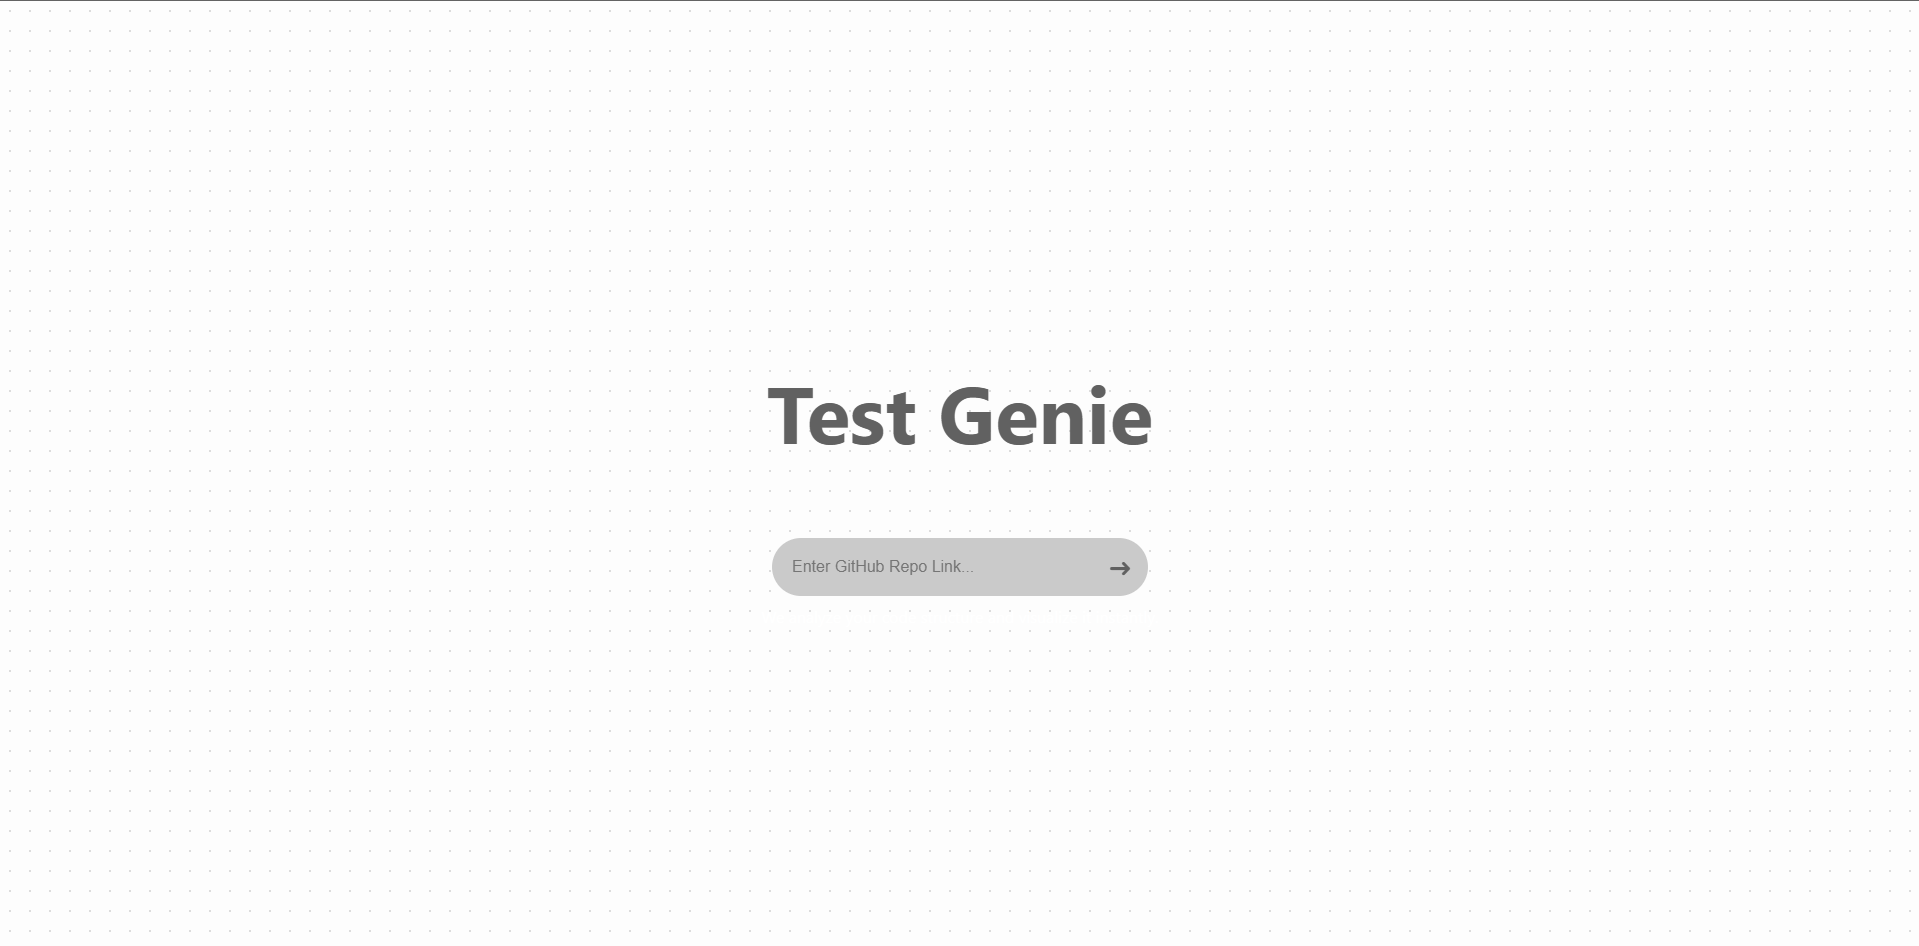
\includegraphics[width=0.8\textwidth]{images/homepage.png}
    \caption{Homepage of Test Genie system.}
    \label{fig:homepage}
\end{figure}

Main Features:
\begin{itemize}
    \item \textbf{Git project repo link input field:} Users can input the URL of their Git project repository to analyze.
\end{itemize}
\subsection{Interactive Dependency Diagram}

The dependency diagram is one of the core components of the Test Genie system. It visualizes to users the relationships between blocks in a project, such as files, functions, and classes.

\begin{figure}[H] 
    \centering
    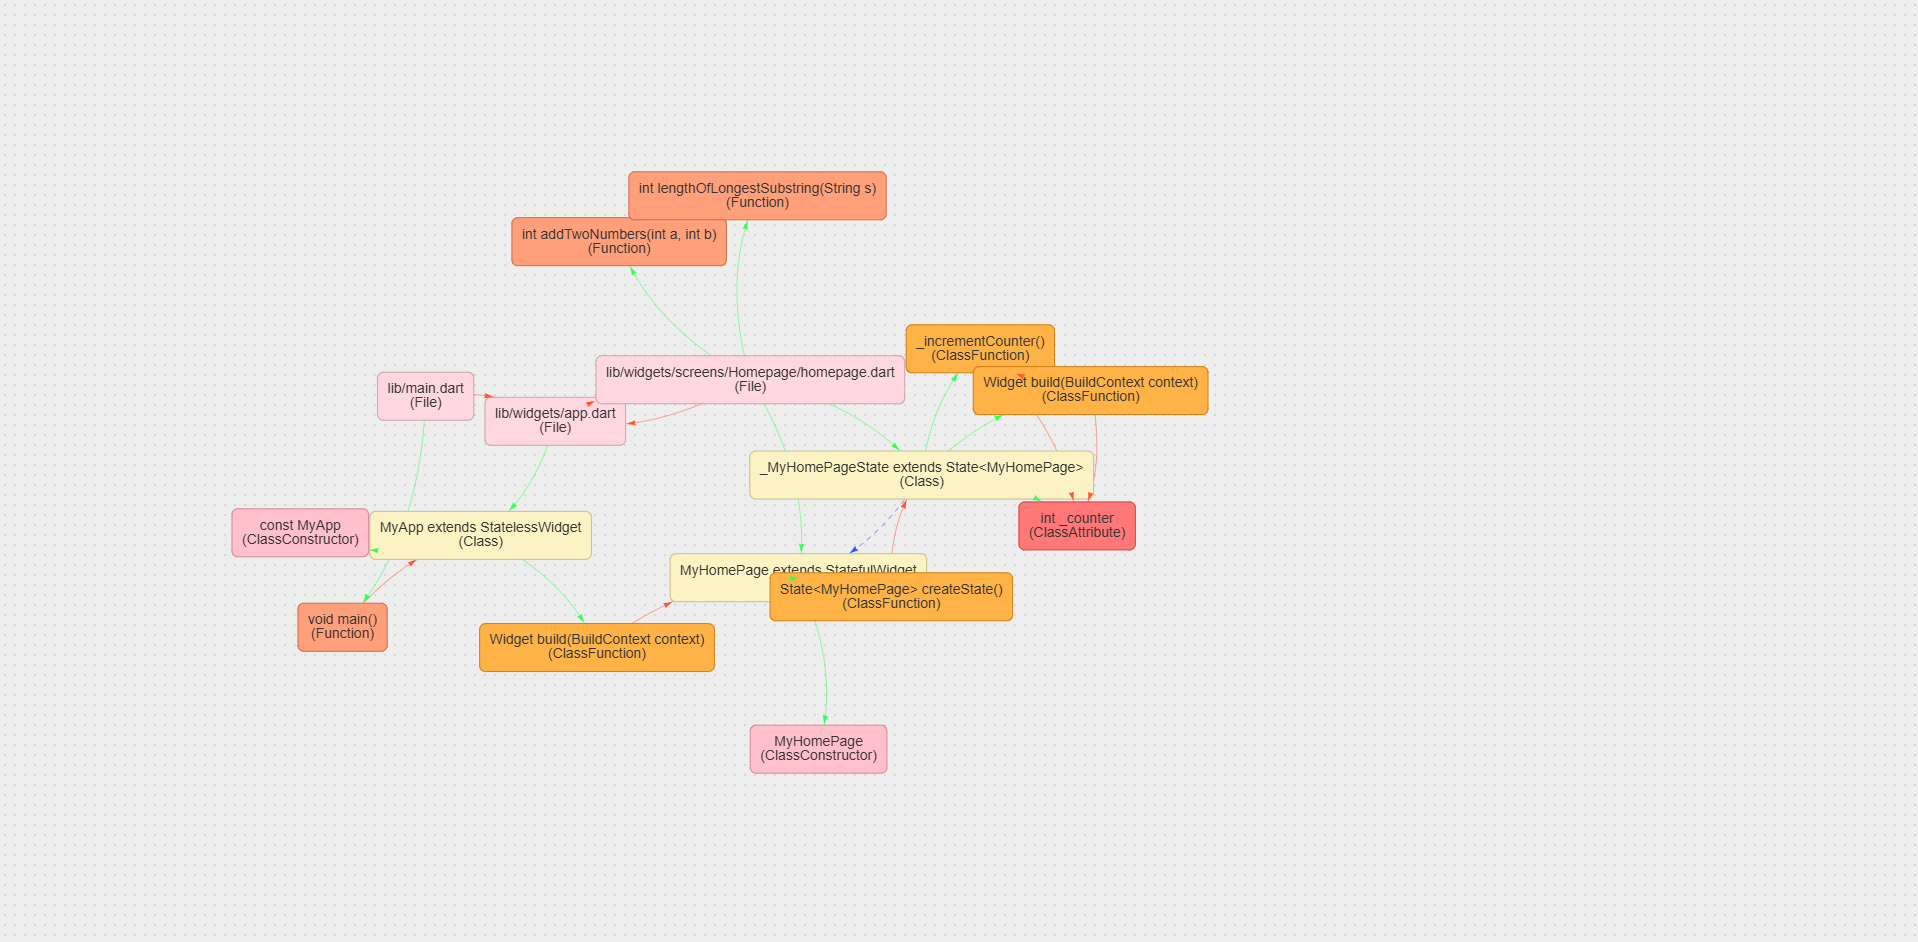
\includegraphics[width=0.8\textwidth]{images/diagram-initial_load.png}
    \caption{Initial load of the dependency diagram.}
    \label{fig:diagram-initial_load}
\end{figure}

\begin{figure}[H]
    \centering
    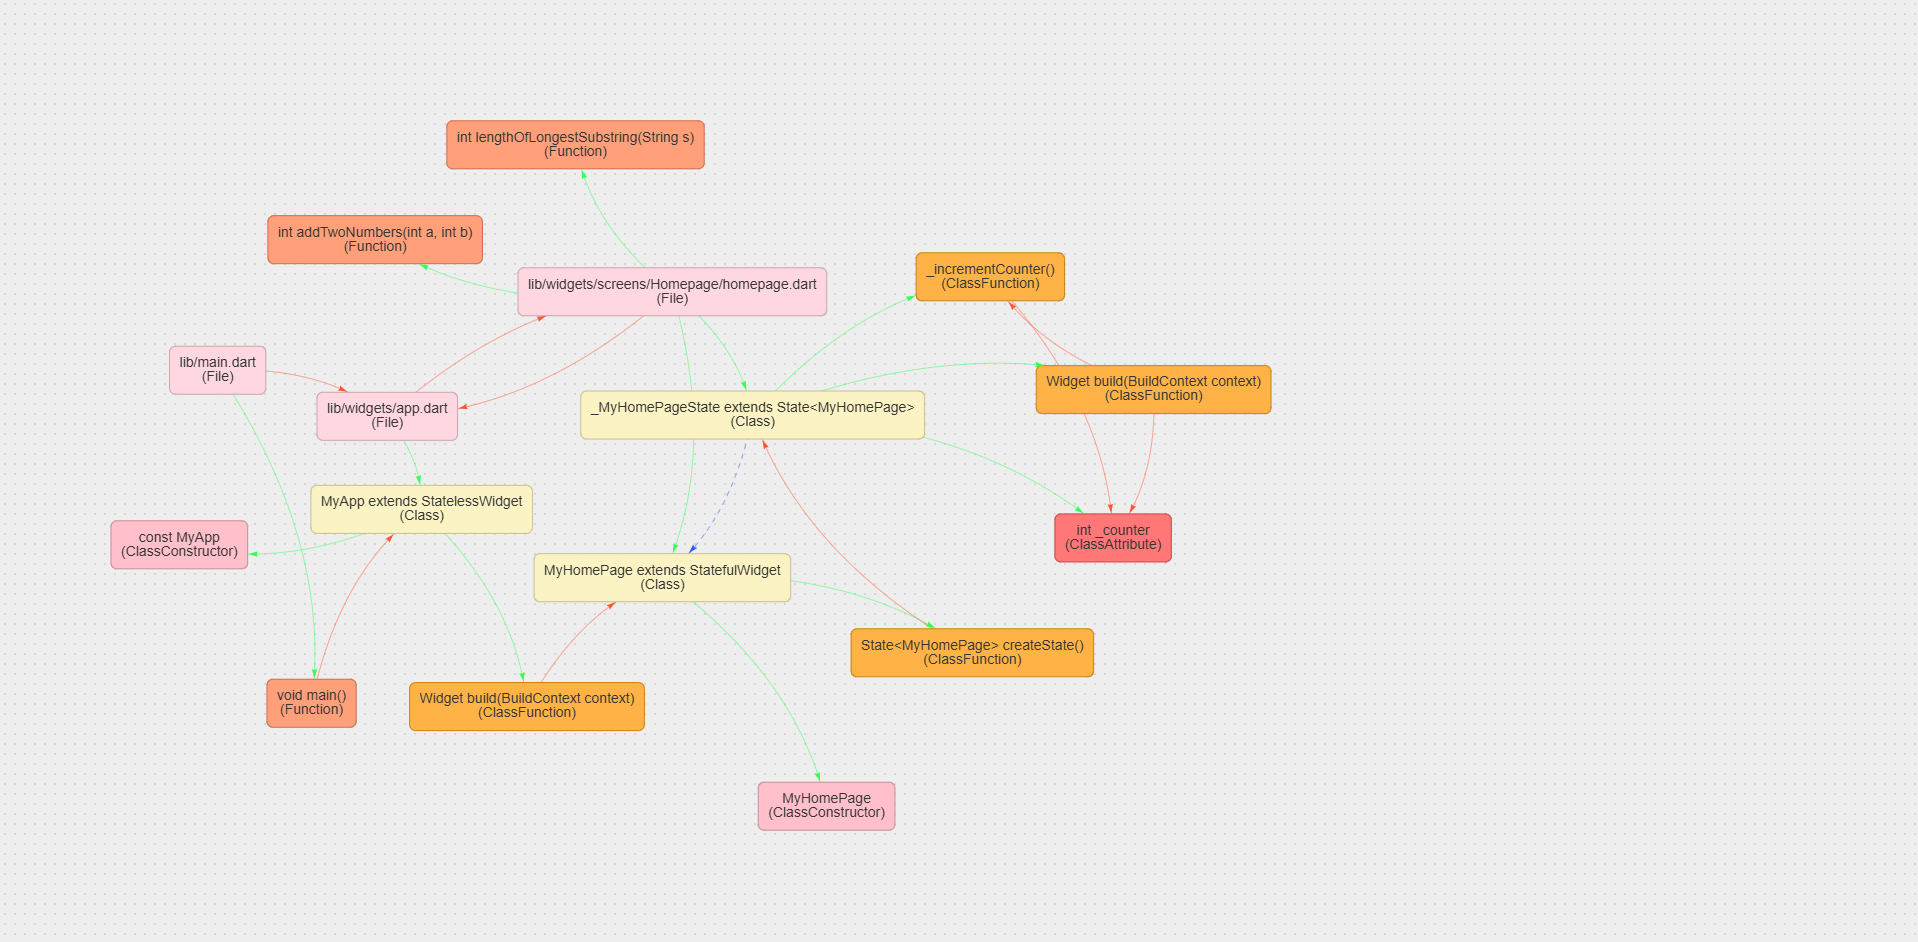
\includegraphics[width=0.8\textwidth]{images/diagram-dragged.png}
    \caption{Diagram blocks can be dragged to rearrange their positions.}
    \label{fig:diagram-dragged}
\end{figure}

Key Interactions:
\begin{itemize}
    \item \textbf{Drag and Drop:} Users can click and drag blocks to rearrange them for better visualization (Figure~\ref{fig:diagram-dragged}).
    \item \textbf{Zoom and Pan:} The diagram supports zooming in and out for detailed or high-level views. Users can pan the diagram to focus on specific areas.
    \item \textbf{Click on Block:} Clicking a block opens its details, including content (source code), predictions, and test cases.
\end{itemize}

\subsection{Block Detail View}

When a block in the diagram is clicked, the Block Detail View is displayed (Figure~\ref{fig:block-detail}). This view provides detailed information about the selected block.

\begin{figure}[H]
    \centering
    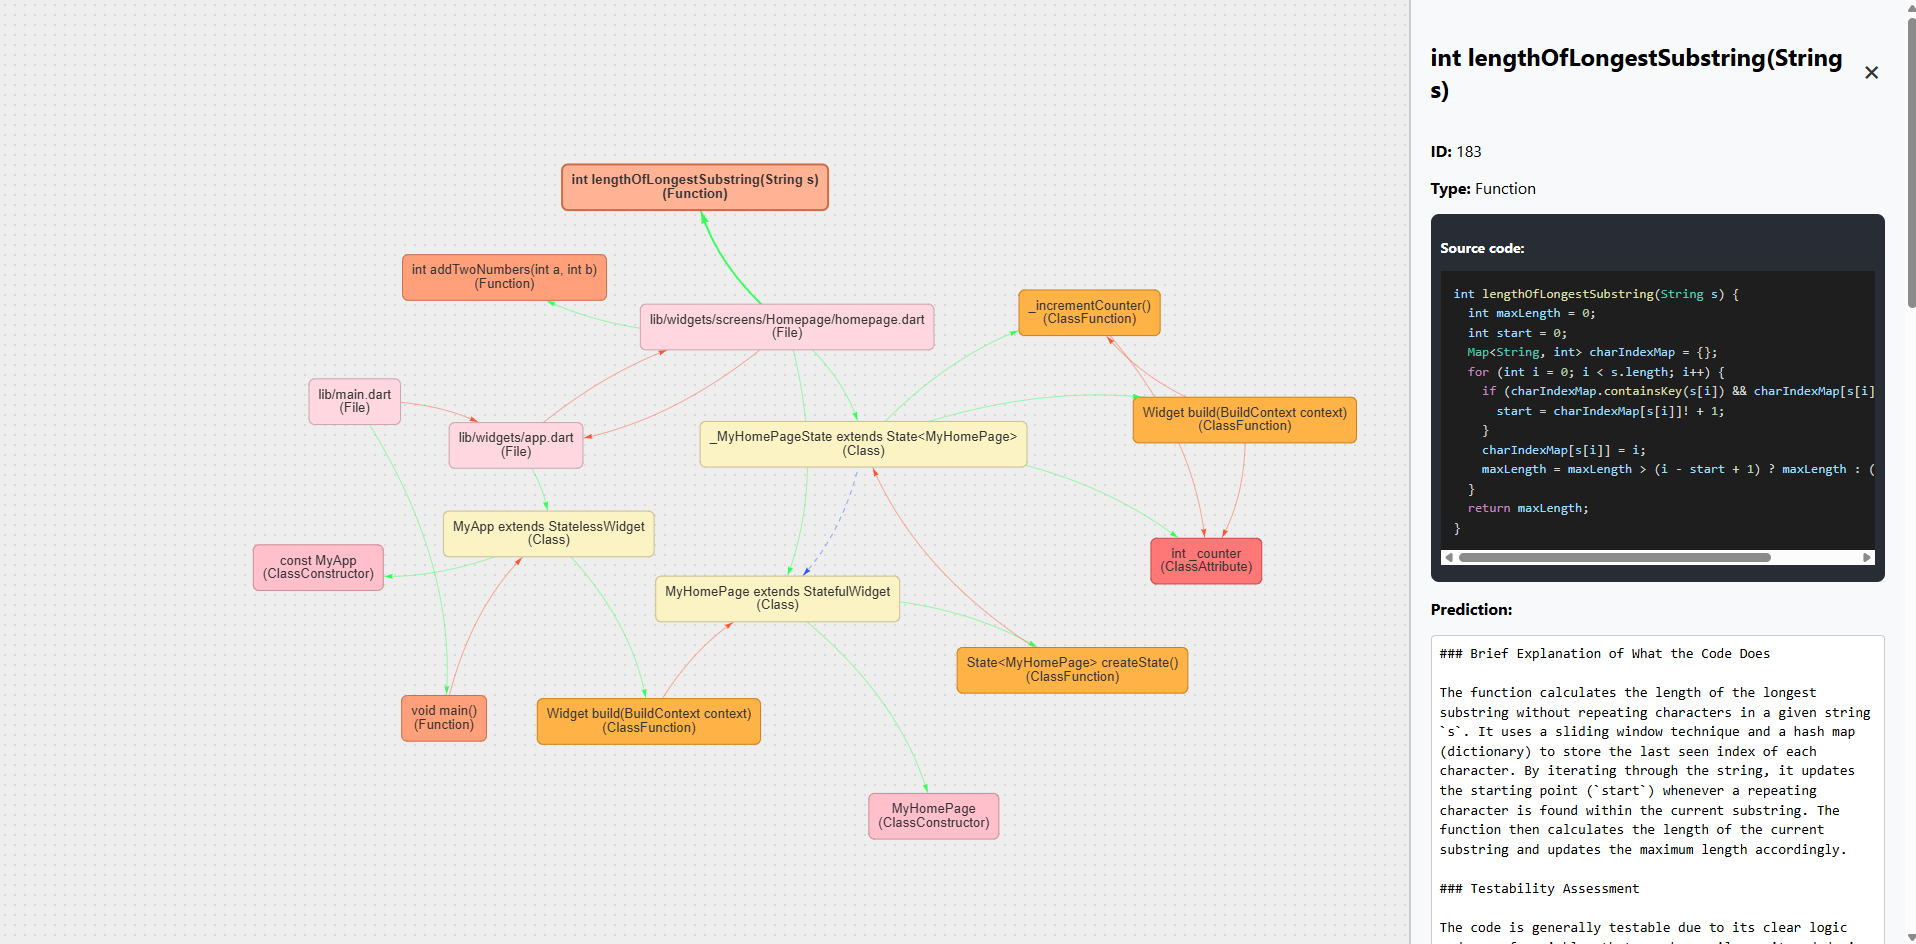
\includegraphics[width=0.8\textwidth]{images/block_detail.png}
    \caption{Block Detail View showcasing the block's content and prediction.}
    \label{fig:block-detail}
\end{figure}

Key Features:
\begin{itemize}
    \item \textbf{Source Code Content:} Displays the source code content of the block.
    \item \textbf{Prediction:} Shows the AI-generated prediction for the block's functionality.
    \item \textbf{Adjustable Prediction:} Users can modify the prediction to refine its accuracy.
    \item \textbf{Test Case Viewer:} Displays the associated test cases for the block, if available.
\end{itemize}

\subsection{Adjustable Predictions}

One of the unique features of Test Genie is the ability to adjust AI-generated predictions. Figure~\ref{fig:prediction-adjustable} showcases how users can interact with and modify predictions.

\begin{figure}[H]
    \centering
    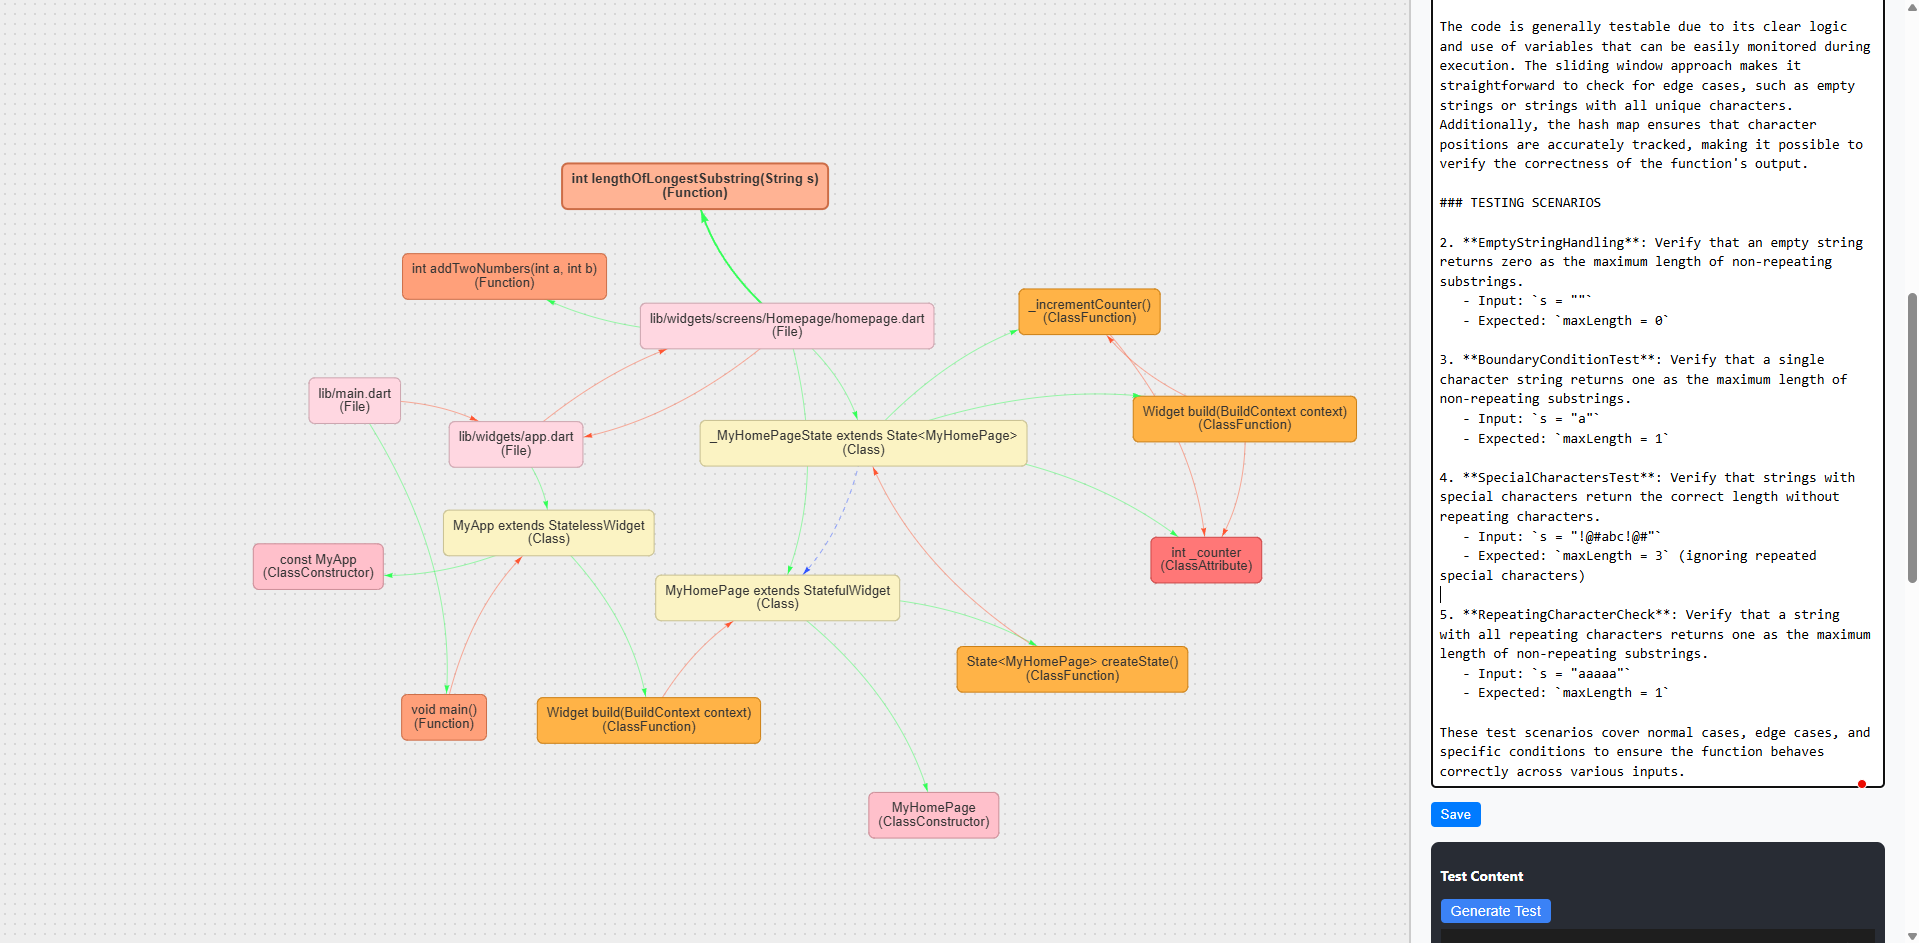
\includegraphics[width=0.8\textwidth]{images/prediction-adjustable.png}
    \caption{Prediction adjustment interface for refining AI-generated predictions.}
    \label{fig:prediction-adjustable}
\end{figure}

Key Features:
\begin{itemize}
    \item \textbf{Editable Text Field:} Users can directly edit the prediction to increase its accuracy.
    \item \textbf{Save Button:} Saves the updated prediction to the database.
\end{itemize}

\subsection{Test Generation}

After analyzing the blocks, Test Genie allows users to generate test cases for specific blocks. Users can view the generated test cases and validate them.

\begin{figure}[H]
    \centering
    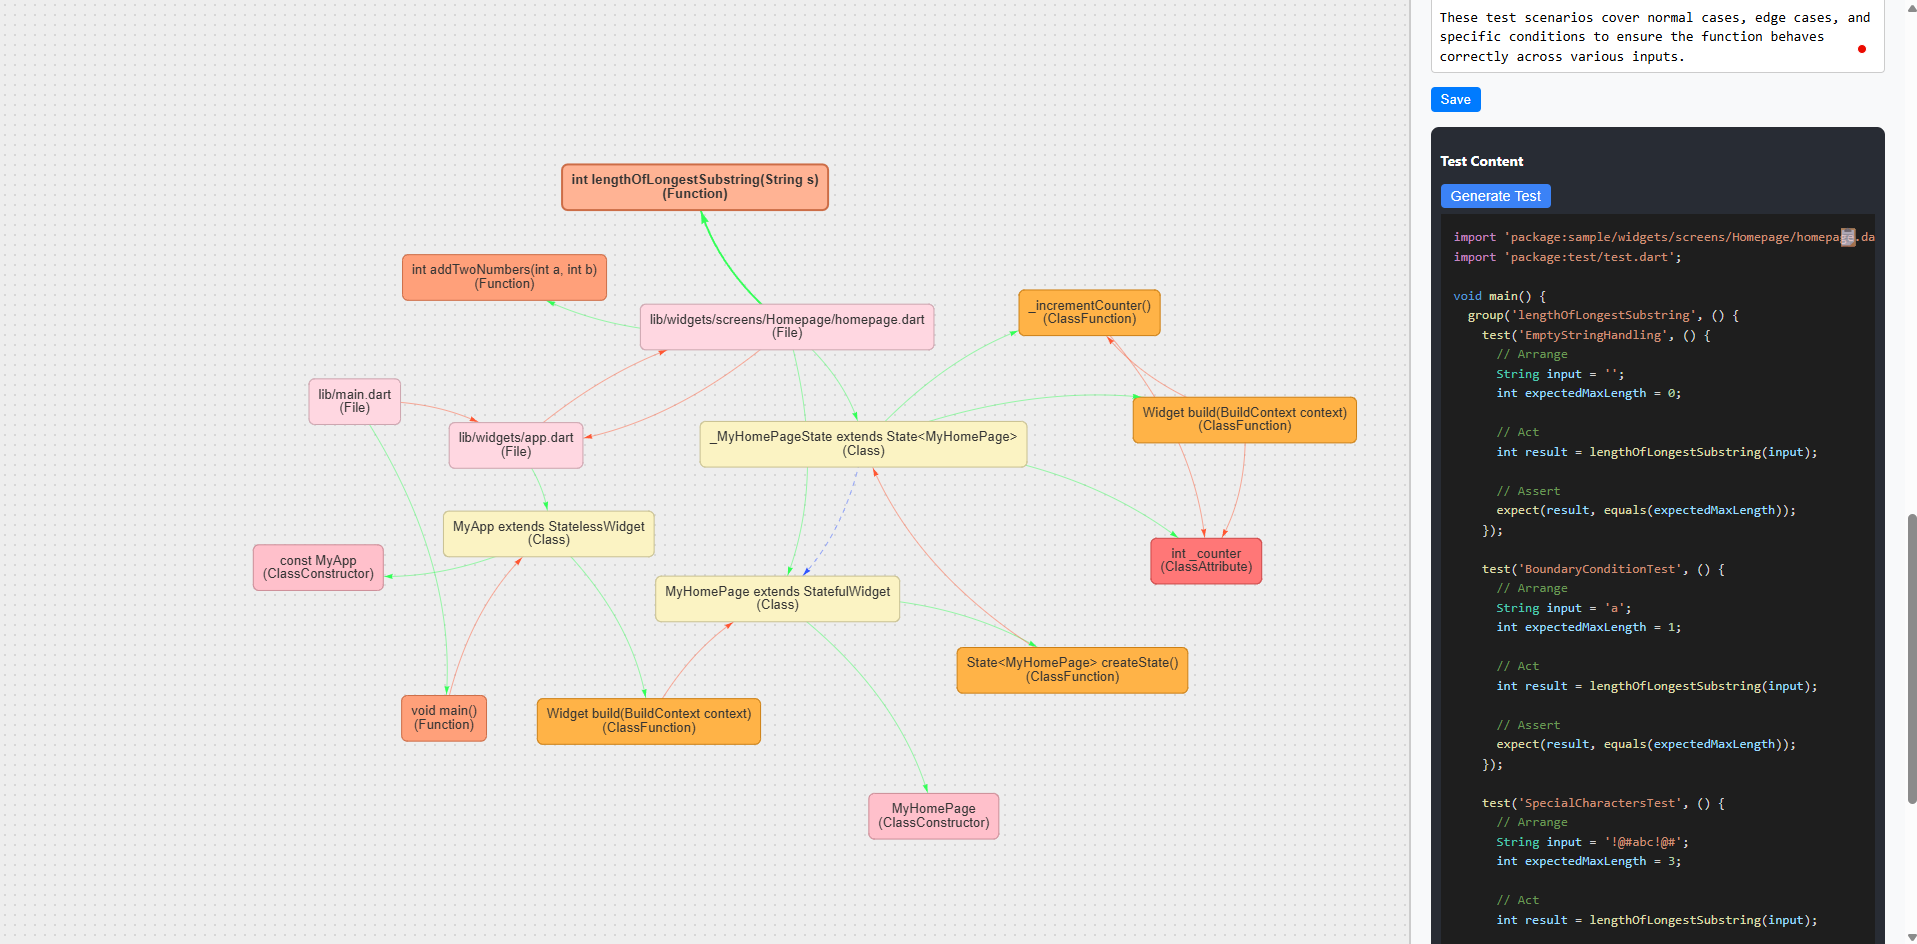
\includegraphics[width=0.8\textwidth]{images/generated_test.png}
    \caption{Generated test cases for a specific block.}
    \label{fig:generated-test}
\end{figure}

Key Features:
\begin{itemize}
    \item \textbf{View Test Cases:} Displays the generated test cases for the selected block.
    \item \textbf{Quick copy button:} Allows users to quickly copy the test case code to the clipboard for easy integration into their projects.
\end{itemize}

\subsection{Summary of Interactions}

The Test Genie system combines a user-friendly interface with advanced functionalities to simplify the process of dependency analysis and test generation. By integrating interactive diagrams, adjustable predictions, and robust test generation, it provides a comprehensive solution for software analysis and testing.